\section{Results}

\subsection*{Population dynamics}
\begin{figure}[H]
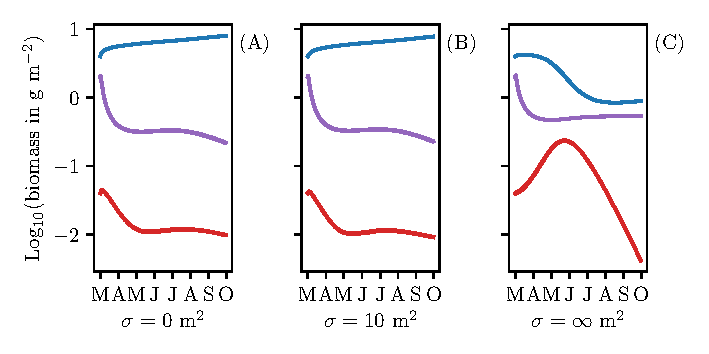
\includegraphics{plots/populations.pdf}
\caption{Total populations of consumers \emph{(blue)}, predators, \emph{(red)} and resources \emph{(purple)} from 1st of april to 1st of october. We vary the rationality, from total rationality \emph{(1)}, bounded rationality ($\sigma = 10$), \emph{(2)} and fully irrational, $\sigma = \infty$, \emph{(3)}, corresponding to a simple Lotka-Volterra model.}
\label{fig:long_term_populations}


\end{figure}
The difference in population dynamics between a system with no behavioral optimization and full rationality \Cref{fig:long_term_populations}(1,3) is stark, where the system with bounded rationality has approximately the same dynamics as the one . The resources reach a stable level quickly in all three cases, but the populations of consumers and predators differ markedly. The difference in populations between the system with bounded rationality \Cref{fig:long_term_populations}(2) and the fully rational system appears to be negligible, \Cref{fig:long_term_populations}(1). The main driver of the change in population dynamics seems to be the ability to retreat to a refuge, and not the exact shape of the distributions when interacting.

\subsection*{Bounded rationality and full rationality}
\begin{figure}[H]
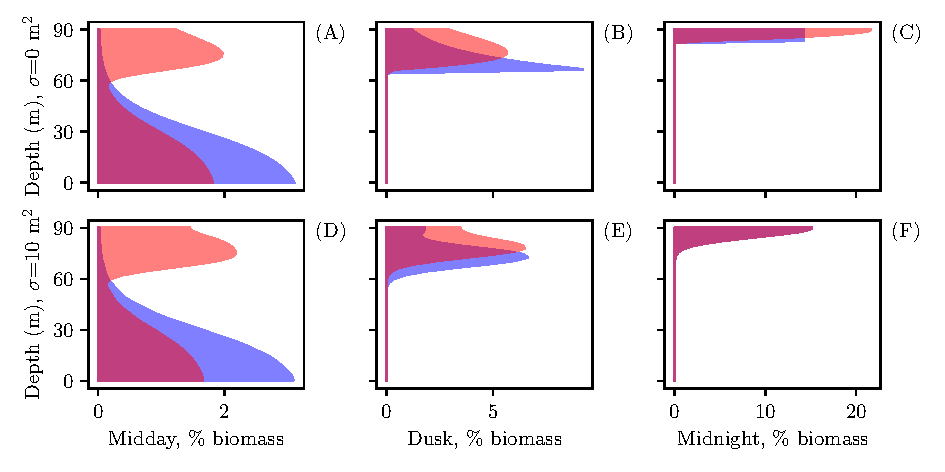
\includegraphics{plots/both_specific_dists.pdf}
\caption{Daily distribution of consumers \emph{blue} and predators \emph{red} at noon \emph{(A,D)}, dusk \emph{(B,E)} and at midnight, \emph{(C,F)} with full (A-C) and bounded rationality (D-F) on the 22nd June (Summer solstice)}
\label{fig:both_specific_dists}
\end{figure}
At noon, \Cref{fig:both_specific_dists}(A) the consumers form a deep scattering layer, where most of the predators are also present, excepting a few hanging out higher in the water column deterring upward consumer migration \Cref{fig:specific_dists_rational}(1)(15 m), corresponding to the modelling results of \citep{jerome}. At dusk, \Cref{fig:both_specific_dists}(B) the predators have a greater concentration near the surface, while the consumer "box" is begining to form, yet still with a continuous drop-off to the surface due to the risk from the light. At midnight \Cref{fig:both_specific_dists}(C) the consumers are concentrated near the surface, with a discontinuous drop to nothing. The predators follow the consumers, albeit with a continuous shape, both distributions being similar to the results of \citep{verticalmigration}.

Examining snapshots of the migration in the ecosystem with bounded rationalty, \Cref{fig:specific_dists_irrational}(D-F), we see roughly the same picture as in \Cref{fig:specific_dists_rational}(A-C). The greatest difference is at midnight and dusk, \Cref{fig:specific_dists_irrational}(B,E,C,F), where the bounded rationality leads to a smooth shape for the distrbution of consumers. At noon, the distributions in the system with bounded rationality \Cref{fig:specific_dists_irrational}(D) and perfect rationality \Cref{fig:specific_dists_rational}(A) are almost entirely equal.

\subsection*{Seasonal variation}
\begin{figure}[H]
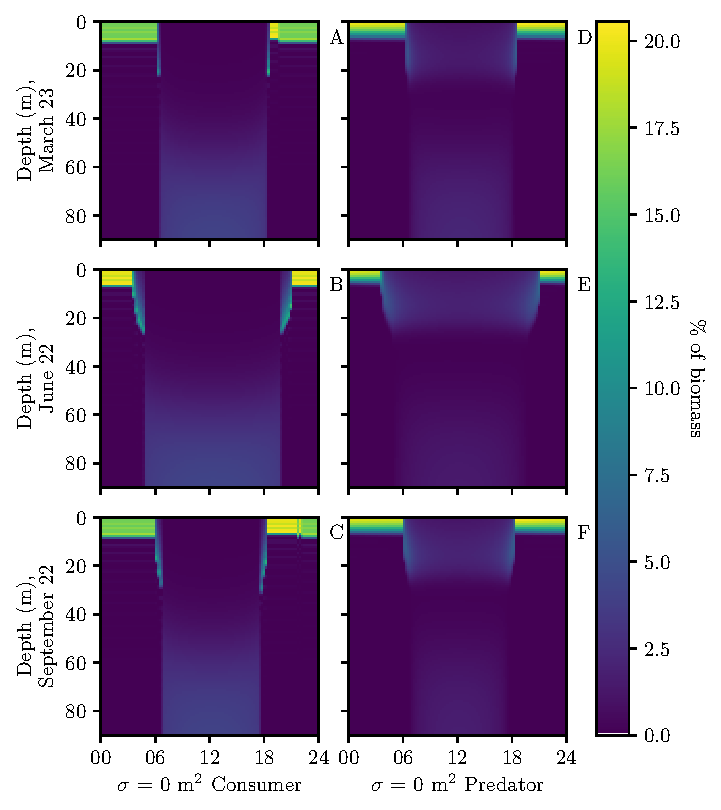
\includegraphics{plots/total_heatmap.pdf}
\caption{Vertical distribution of consumers \emph{(A-C)} and predators \emph{(D-F)} at spring equinox (March 22), summer solstice (June 22) and fall equinox (September 23)}
\label{fig:heatmap_total}
\end{figure}
%To understand the migration in greater detail, we look at the complete migration picture.
The vertical migration pattern, \Cref{fig:heatmap_total} is apparent throughout the seasons. Both consumers and predators are highly concentrated at the top of the water column during nighttime, and at day they scatter to the deep. The pattern of the predators \Cref{heatmap_total}(D-F) is slightly different from the consumer pattern, \Cref{fig:heatmap_total} (A-C). At nighttime there is still a non-zero concentration of predators in the upper layers of the water-column, there to catch any errant prey. In the spring \Cref{fig:heatmap_total}(A) the consumer migration is very fast, reflecting relatively fast shift in light levels, with a much slower migration in the summer \Cref{fig:heatmap_total}(B,E).

Moving the hands on the clock forward to October, we see a different pattern \Cref{fig:heatmap_total}(C,F). The migration differs from summer migration, in that the descent and ascent are steeper, and the distributions are wider during the night.

\subsection*{Feeding rates}
\begin{figure}[H]
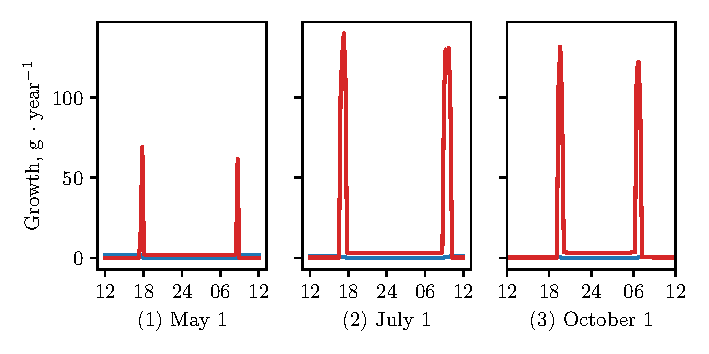
\includegraphics{plots/growth_short_rational.pdf}
\caption{Seasonal comparison of consumer \emph{(blue)} and predator, \emph{(red)} feeding patterns on March 22 (spring equinox) \emph{(A)}, 22 June (summer solstice) \emph{(B)} and 23 of September (fall equinox) \emph{(C)}}
\label{fig:growth_short_rational}
\end{figure}
At all three points in time, consumers have a constant feeding level throughout the night \Cref{fig:growth_short_rational}. The main feeding time for predators is at dawn and dusk, with a slight peak during the day as well, \Cref{fig:growth_short_rational}. The length of predator feeding duration increases with the length of the night,  \Cref{fig:growth_short_rational}(B,C). Peak predator feeding activity decreases by a factor of 3/4 throughout the seasons, \Cref{fig:growth_short_rational}, reflecting lower maximal light levels.
\begin{figure}[H]
  \begin{centering}
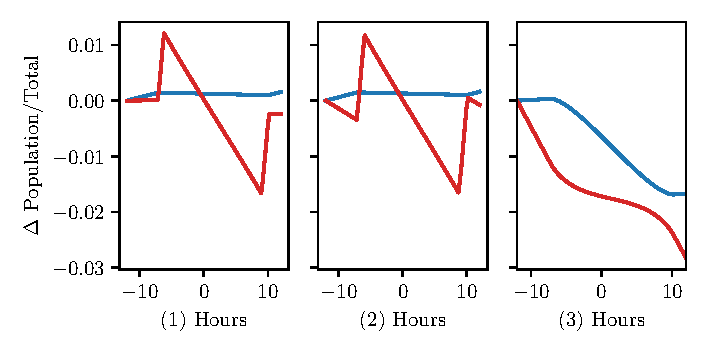
\includegraphics{plots/pop_dyn_comp_full_semi_none.pdf}
\end{centering}
\caption{Comparison of consumer \emph{(blue)} and predator, \emph{(red)} pr. capita growth patterns with complete rationality \emph{(A)}, bounded rationality \emph{(B)} and full irrationality \emph{(C)}}
\label{fig:pop_short_term}
\end{figure}
Looking at short-term population growth in the model with full rationality and bounded rationality, \Cref{fig:pop_short_term}(A,B), the change in consumer and predator populations throughout a day is on the order of $10^{-3}$. In contrast, the model with constant behavior has rather large fluctuations of populations through a single day \Cref{fig:pop_short_term}(C).


%Compare to behavior visser2001observations, hay1991zooplankton

%Compare to wang2014seasonal, klevjer2016large, olivar2017mesopelagic, beaugrand2001geographical, colebrook1979continuous

%%% Local Variables:
%%% mode: latex
%%% TeX-master: "main"
%%% End:
